\documentclass[11pt,letterpaper]{article}
\usepackage[margin=1in]{geometry}
\usepackage{amsmath,amssymb,graphicx,booktabs,longtable,array}
\usepackage{xcolor,listings}
\usepackage[hidelinks]{hyperref}
\graphicspath{{figures/}}
\setlength{\parindent}{0pt}
\setlength{\parskip}{0.55em}
\setlength{\emergencystretch}{2em}
\newcommand{\E}{\mathbb{E}}
\newcommand{\softmax}{\operatorname{softmax}}
\newcommand{\LSE}{\operatorname{logsumexp}}
\lstset{basicstyle=\ttfamily\small,breaklines=true,columns=fullflexible,
  frame=single,rulecolor=\color{black!20},backgroundcolor=\color{black!2},
  showstringspaces=false,aboveskip=0.7em,belowskip=0.7em}
\title{Cue Specificity and Contour Completion\\
\large Comparing counted, Hebbian, and Hopfield priors with VSA image evidence}
\author{}
\date{20 November 2026}
\begin{document}
\maketitle
\vspace{-1.5em}

\section{Essential terms}
The terms below refer to the computational experiment described in this report.
\begin{longtable}{@{}p{0.19\linewidth}p{0.76\linewidth}@{}}
\toprule
Term & Meaning in this experiment \\
\midrule
\endhead
Feature or factor & One variable describing a drawing, such as nose shape, ear shape, or feature layout. Each has a small set of predefined values. \\
Recipe, $z$ & A complete list of feature values that specifies one drawing. For example, a wide head, long ears, wide eye spacing, a muzzle, aligned layout, and dot eyes. \\
Candidate & A recipe being considered as an explanation of the observed image. Rendering that recipe produces its candidate image. \\
Renderer, $R$ & The fixed program that turns a recipe into a binary line drawing. It defines what each supplied feature in the recipe looks like. \\
Observation, $y$ & The partial, noisy image presented to the model. Stroke pixels have value 1 and background pixels have value 0. \\
Visibility mask, $M$ & A binary array identifying which pixels were observed. A hidden pixel is unknown, whereas visible background is evidence that a stroke is absent. \\
Encoder & A mapping from image pixels to a representation used for inference. The current image encoder uses fixed random scheme for converting pixel positions to high dimensional vectors. A learned, cue-modulated encoder is discussed at the end. \\
Codebook & A collection of fixed vectors assigned to positions or feature values. A code supplies a consistent representation for its assigned item. \\
VSA & Vector symbolic architecture. Here, binding combines role and position codes, and superposition adds many encoded contributions into one vector. \\
Prior, $p(z)$ & A distribution over recipes learned before the test image is presented. The tested priors learn recipe familiarity through feature counts, exemplar similarity, Hebbian updates, or Hopfield energy. \\
Prior cue, $c$ & Extra information supplied during testing. A category cue changes the category-based prior. A direct feature cue adds evidence such as ``the nose is round.'' The two cue procedures are specified separately below. \\
Evidence / likelihood & How well a candidate's predicted visible pixels match the observation under the assumed noise process. The VSA backend approximates this score using vector distance. \\
Posterior, $q(z)$ & The normalized distribution over recipes after combining image evidence with the selected prior and any cue. \\
MAP sketch & The rendering of the single recipe with the highest posterior probability. MAP means maximum a posteriori. \\
Posterior-mean drawing & A pixelwise weighted average of candidate renderings, using their posterior probabilities. Grey regions indicate uncertainty among candidate drawings. \\
Training / inference & Training fits a prior from complete synthetic examples, with labels available to some methods. Inference estimates the recipe of a new partial image using the fitted prior. \\
\bottomrule
\end{longtable}
\addtocounter{table}{-1}

\section{Question and scope}
The motivating question is how much contextual information is needed for an ambiguous image to support a meaningful part interpretation, such as identifying a patch as a muzzle. Mooney images provide a related setting in which knowledge can change the interpretation of an unchanged two-tone stimulus \cite{schwiedrzik2018,lazarova2025}.

The implemented experiment first asks a more controlled question. Given a supplied feature vocabulary and renderer, how do learned priors and supplied cues affect recovery of missing facial features? We compare alternative priors on the same masked images and use controlled masks to test when a cue can change what the model fills in. The final discussion develops the broader encoder-learning question.

The stimuli are synthetic line drawings with a known visibility mask. Their missing pixels are explicitly identified. A thresholded photograph also changes which boundaries and regions are available, but supplies no equivalent missing-pixel mask. The reported results therefore concern a controlled completion task.

\section{Stimuli and training data}
\subsection{The recipe space}
Every recipe has six factors, listed in Table~\ref{tab:factors}. The full Cartesian product contains
\begin{equation}
|\mathcal Z|=3^6=729
\end{equation}
possible complete drawings. Eye shape varies independently of eye spacing. Figure~\ref{fig:face-designs} illustrates all six features using the current renderer.

\begin{table}[htbp]
\centering
\begin{tabular}{ll}
\toprule
Factor & Available values \\
\midrule
Head shape & Round, wide, tall \\
Ear shape & Round, pointed, long \\
Eye spacing & Narrow, medium, wide \\
Nose shape & Triangle, round, muzzle \\
Layout & Aligned, lowered, scrambled \\
Eye shape & Dots, arches, oval pupils \\
\bottomrule
\end{tabular}
\caption{The supplied feature vocabulary. Each rendered image is $40\times40$ pixels.}
\label{tab:factors}
\end{table}

\begin{figure}[htbp]
\centering
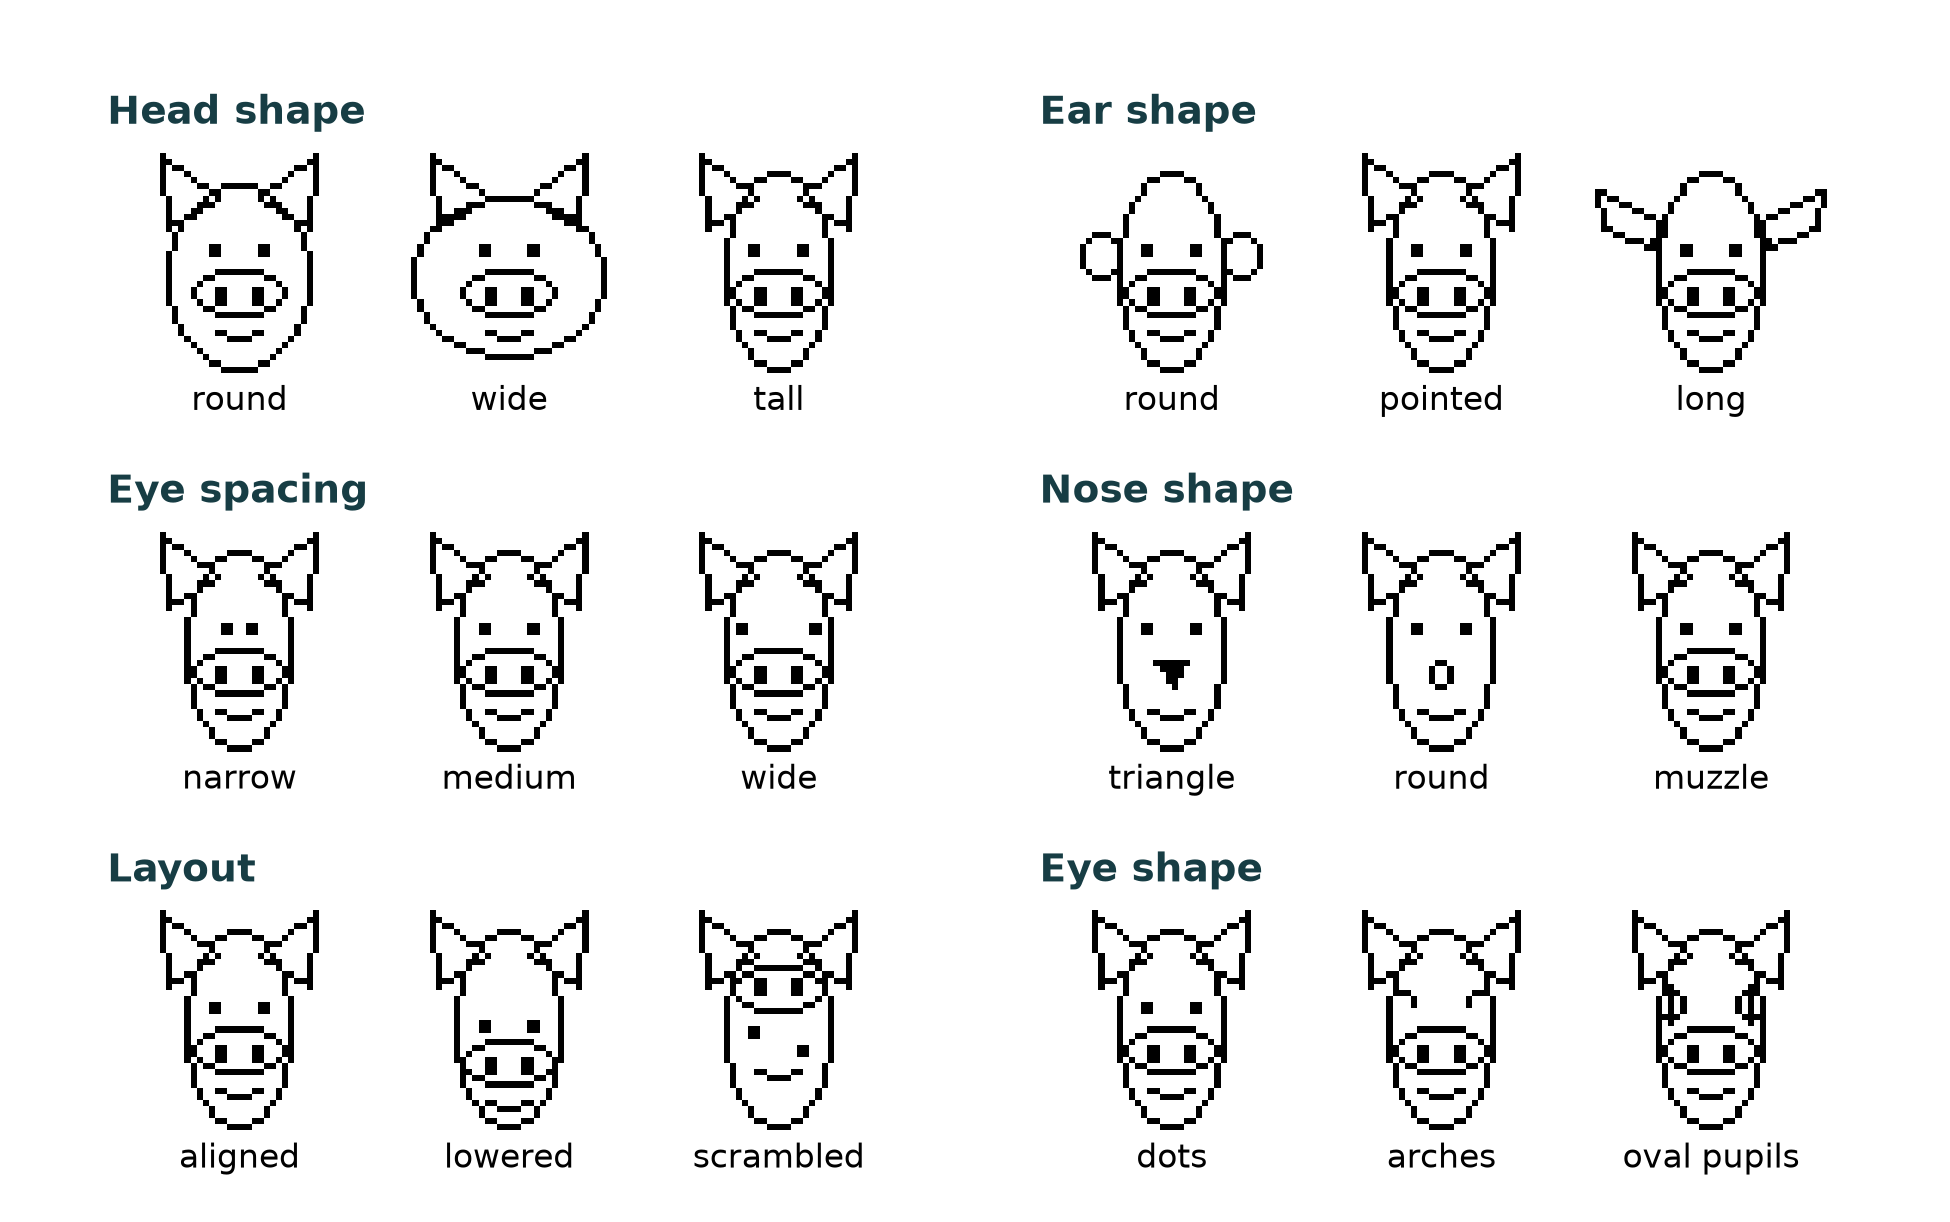
\includegraphics[width=\linewidth]{face_designs.png}
\caption{The current face designs. Within each group, one feature changes while the other five stay fixed.}
\label{fig:face-designs}
\end{figure}

\subsection{Training and held-out combinations}
The recipe space is split before sampling training examples. With split seed 7, 547 recipes are available for training and 182 are held out. The renderer can represent all 729, including the held-out combinations.

A synthetic data generator defines overlapping cow-like, cat-like, and human-like sampling distributions. Morphological features have preferred values. Dot eyes are common in cow-like examples, oval pupils in cat-like examples, and arches in human-like examples. We sample 250 examples per category with replacement using training seed 11. The 750 training draws contain 261 distinct recipes. All methods receive the sampled recipes. The within-category count and supervised Hebbian methods also receive the category labels. The generator's probability tables determine sampling.

The category names identify sampling distributions. A particular drawing can combine features typical of different groups. A held-out drawing is a new combination of known feature values, rather than a new primitive or drawing style.

\section{Learning priors over face recipes}
\subsection{Feature counting}
The basic learning operation is to count how often each feature value occurs. For feature $j$ and value $k$, let
\begin{equation}
n_{jk}=\sum_{n=1}^{N}\mathbf 1[z_j^{(n)}=k].
\end{equation}
With $K_j$ possible values and additive smoothing $a=1$, the estimated frequency is
\begin{equation}
\widehat\pi_j(k)=\frac{n_{jk}+a}{N+K_ja}.
\label{eq:counts}
\end{equation}
Smoothing gives every value some probability. For example, eight dot eyes, two arches, and zero oval pupils become probabilities $9/13$, $3/13$, and $1/13$ after adding one to every count.

For a chosen feature set $J$, the factorized count prior is
\begin{equation}
p_J(z)=\prod_{j\in J}\widehat\pi_j(z_j)
\prod_{j\notin J}\frac{1}{K_j}.
\label{eq:pooled}
\end{equation}
The rule selecting features and multiplying their probabilities is supplied by the implementation. Training learns the frequencies used by that rule.

In the array representation, each row of \texttt{samples} is a training recipe and each row of \texttt{states} is a candidate recipe. The following block counts training values, converts them into log probabilities, and looks up the appropriate value for every candidate.
\begin{lstlisting}[language=Python]
counts = np.bincount(samples[:, j], minlength=K_j) + 1.0
log_probabilities = np.log(counts / counts.sum())
candidate_log_scores += log_probabilities[states[:, j]]
\end{lstlisting}
Thus, \texttt{samples[:, j]} supplies values to count, while \texttt{states[:, j]} supplies values to score.

\subsection{Count-based baselines}
\textbf{Uniform vocabulary.} Every recipe receives $p(z)=1/729$. Its preference comes entirely from the image evidence and the supplied candidate vocabulary.

\textbf{Layout.} Equation~\eqref{eq:pooled} uses only layout frequencies. Head shape, ear shape, eye spacing, nose shape, and eye shape receive uniform weights.

\textbf{Latent categories.} Let $G=\{\text{cow-like},\text{cat-like},\text{human-like}\}$ be the set of face categories. Each $g\in G$ describes the type of face a recipe represents. To estimate $p(z\mid g)$, we count feature values among training faces labeled $g$. When the category is unknown, we average the recipe probabilities over all categories:
\begin{equation}
p(z\mid g)=\prod_j\widehat\pi_{jg}(z_j),\qquad
p_{\mathrm{category}}(z)=\sum_{g\in G}\widehat w_g\,p(z\mid g).
\label{eq:category}
\end{equation}
The mixture weights $\widehat w_g$ are smoothed category frequencies. Since training draws are balanced, they are equal here. Features are independent within each category model, while mixing categories creates dependencies between features. Wide heads and long ears can increase the relative contribution of the cow-like component, which in turn changes support for nose values.

\subsection{Training exemplars}
The exemplar prior scores a recipe by its similarity to complete recipes seen during training. The Hamming distance $d_H$ counts the feature values that differ. An exemplar contributes $e^{-\gamma d_H}$ to the candidate score,
\begin{equation}
p_{\mathrm{ex}}(z)\propto \frac{1}{N}\sum_{n=1}^N
  e^{-\gamma d_H(z,z^{(n)})},\qquad \gamma=2.5.
\end{equation}
Repeated examples contribute each time they occur. The normalizer sums the scores over all 729 recipes.

\subsection{Supervised Hebbian learning}
Represent feature value $k$ with the indicator $a_{jk}=\mathbf 1[z_j=k]$ and category $g$ with $s_g=\mathbf 1[\text{label}=g]$. The connection from a feature value to its category strengthens when both are active,
\begin{equation}
W_{gjk}\leftarrow W_{gjk}+\eta s_g a_{jk},
\qquad C_g\leftarrow C_g+\eta s_g.
\end{equation}
Each $W_{gjk}$ and $C_g$ starts at one. Normalizing across values of feature $j$ gives $\widehat\pi_{jg}(k)=W_{gjk}/\sum_l W_{gjl}$, and normalizing the category totals gives $\widehat w_g=C_g/\sum_h C_h$. These define the same mixture as Equation~\eqref{eq:category}. With one pass and $\eta=1$, each update adds one occurrence. The supervised Hebbian prior thus implements smoothed frequency counting as a local learning rule.

\subsection{Label-free competitive Hebbian learning}
Three units learn recurring combinations from the same mixed training examples. Each unit $u$ starts with random tables $W_{ujk}$ that sum to one across the values of each feature. With current mixture weight $\pi_u$ and recent usage $r_u$, its response to a face is
\begin{align}
b_u(z) &= \sum_j \log W_{uj,z_j}+\log\pi_u-\lambda\log(3r_u),\\
s_u &= \softmax_u(b/T),\\
W_{ujk} &\leftarrow W_{ujk}+\eta s_u(a_{jk}-W_{ujk}).
\label{eq:competitive}
\end{align}
A unit that already matches the face tends to respond more strongly and moves its weights further toward the observed features. The usage term encourages underused units to compete. An exponential moving average with rate $0.02$ tracks usage, and accumulated responsibilities give the mixture weights. With a starting pseudocount of one per unit, the fitted prior is $p_{\mathrm{comp}}(z)=\sum_u\pi_u\prod_j W_{uj,z_j}$. The matched comparisons use 20 passes, $\eta=.03$, $T=.7$, $\lambda=2$, and initialization seeds 0, 1, and 2. The units learn from co-occurrence and receive no category labels.

\subsection{Hopfield energy prior}
Each complete recipe is encoded as an 18-entry bipolar vector $x(z)$, with one $+1$ for the selected value and two $-1$s per feature. The Hopfield weights store pairwise correlations across complete training recipes,
\begin{equation}
J_{ab}=\frac{1}{18N}\sum_{n=1}^N x_a(z^{(n)})x_b(z^{(n)})\quad(a\ne b),
\qquad J_{aa}=0.
\end{equation}
The energy and the resulting prior are
\begin{equation}
E(z)=-\tfrac12 x(z)^{\mathsf T}Jx(z),
\qquad
p_{\mathrm{H}}(z)=\frac{\exp[-\tau E(z)]}{\sum_{z'}\exp[-\tau E(z')]}.
\end{equation}
Lower energy gives higher prior probability. The comparison evaluates energy on all valid recipes and uses $\tau=1$ by default. The separate Hopfield retrieval demonstration updates feature slots while clamping any supplied feature values. That process can settle in a local energy minimum. In the comparison, MAP selection scores every recipe using image evidence and hints as well as the energy prior.

\subsection{What remains fixed during testing}
\texttt{PriorBank.logpriors} stores one array of log probabilities per prior condition, with one entry per recipe. The arrays remain fixed during testing. Posteriors and iterative feature probabilities are stored separately.

Log scores are normalized by subtracting their log-sum-exp,
\begin{equation}
\operatorname{normalize\_logp}(s)_z
=s_z-\log\sum_{z'}\exp(s_{z'}).
\end{equation}
Exponentiating this result gives probabilities that sum to one.

\section{From visible pixels to evidence scores}
\subsection{Masking and noise}
For a clean drawing $x=R(z^*)$, a visibility mask $M$ is generated and visible pixels are independently flipped with probability $\rho=0.05$. A flipped background pixel becomes a stroke and a flipped stroke becomes background. The displayed observation sets hidden pixels to zero, while $M$ records that these values are unknown.

Random masks use $5\times5$ blocks. Each block is visible with a requested probability $v$. The realized visible fraction, $\sum_iM_i/1600$, varies across seeds. Masks at different $v$ values in the seed sweep use the same underlying random field, producing nested visible regions. The flip field is also held fixed within each face/seed pair.

\subsection{Ordinary pixel likelihood}
Flattening a $40\times40$ image into a list of 1,600 pixels preserves every value and its position. Computing a distance takes a further step: it reduces a comparison with one particular candidate to a single number. Under independent flips with a common rate, the number of mismatches carries all the information needed to score that candidate at a fixed mask.
For candidate $z$, the visible mismatch count is
\begin{equation}
d(z)=\sum_i M_i[y_i-R(z)_i]^2.
\end{equation}
Since all image values are binary, a squared difference is one exactly when the pixels disagree. With independent flips, the log likelihood, up to a constant common to candidates, is
\begin{equation}
\ell_{\mathrm{pix}}(z)=-\beta d(z),\qquad
\beta=\log\frac{1-\rho}{\rho}.
\label{eq:pixel}
\end{equation}
Both observation and candidate use the same mask. A candidate stroke over visible background is penalized. A candidate stroke behind the mask receives no direct pixel penalty.

\subsection{The VSA image encoder}
Consider $Y$, $X$, and $r$ as the row, column, and role of a pixel. Each is assigned a fixed random bipolar code (each entry being 1 or -1). Here the role is a placeholder because the pixel is binary, but it is helpful to preserve for future develop of this architecture where each pixel can hold additional information, such as color, gray-scale intensity, or orientation. With $D=512$, the unit-length code for pixel $(u,v)$ is
\begin{equation}
\phi_{uv}=\frac{r_{\mathrm{pixel}}\odot Y_u\odot X_v}{\sqrt D},
\end{equation}
where $\odot$ denotes elementwise multiplication.
Let $H$ be the vector encoding the entire image, $M_{uv}$ representing the visibility of the pixel from the mask (1 as visible and 0 as masked), and $y_{uv}$ representing the pixel value (1 as black and 0 as white), then
\begin{equation}
H(y,M)=\sum_{u,v}M_{uv}y_{uv}\phi_{uv},
\end{equation}
The encoded image has 512 coordinates, compared with 1,600 raw pixels. Pixel values weight the codes before superposition.

The VSA backend substitutes encoded distance into Equation~\eqref{eq:pixel},
\begin{equation}
\widetilde\ell_{\mathrm{VSA}}(z)
=-\beta\left\|H(y,M)-H(R(z),M)\right\|^2.
\label{eq:vsa}
\end{equation}
This is an approximate evidence score or pseudo-likelihood. With $d_i=M_i[y_i-R(z)_i]$ and unit-length pixel codes,
\begin{equation}
\left\|\sum_i d_i\phi_i\right\|^2
=\sum_i d_i^2+2\sum_{i<k}d_i d_k\,\phi_i^\top\phi_k.
\end{equation}
The second term is cross-talk. Orthogonal codes would recover the ordinary squared pixel distance. Random-code overlap can increase or decrease individual scores. Higher dimension reduces typical overlap at fixed load, but carries no built-in rule that nearby strokes should form a common contour.

The renderer supplies the feature-to-pixel mapping. The encoder's fixed coordinate codes supply a compact representation for comparing those predicted pixels with the observation. The feature labels are already defined by the recipes.

\section{Inference and cue manipulations}
\subsection{How much evidence does an encoded distance provide?}
At a 5\% flip rate, one additional pixel mismatch divides the pixel likelihood by 19. The current VSA score gives one additional unit of squared encoded distance the same penalty. To examine that assumption, first keep the learned prior and hint reliability fixed and write the candidate score as
\[
 w\,\widetilde\ell_{\mathrm{VSA}}(z)+\log p(z)+\log p(c\mid z).
\]
Here $c$ denotes any supplied hint, and its term drops out on uncued trials. The reported VSA runs use $w=1$. A proposed calibration would estimate $w$ on separate uncued observations by minimizing the negative log posterior probability of the true recipe, using the recipe distribution of the calibration sample as the prior. Evaluate the fixed weight on fresh observations. The later sweep of $\alpha$ asks how decisions respond to changing the learned prior.

\paragraph{What dimension changes.}
For this encoder, distinct pixel codes have zero expected inner product over random codebooks. Thus for a fixed image difference the expected squared encoded distance equals the pixel mismatch count at every $D$. Independent code coordinates average out cross-talk as $D$ grows. A fixed codebook can distort different comparisons in opposite directions. Dimension affects the spread of the errors and by itself specifies no scalar correction. Li and colleagues derive distance distributions for independent random projections \cite{li2006}. The shared row and column factors here require their own error analysis.

\paragraph{A likelihood from the observation model.}
For a fixed mask, let $n$ be the visible pixel count and let $A$ contain the corresponding pixel codes as columns. If $b$ is a possible visible binary image and $k_z(b)$ its mismatch count against recipe $z$, the exact probability of observing encoded vector $h$ follows by summing over compatible images:
\[
 P(H=h\mid z,M,A)=
 \sum_{\{b\in\{0,1\}^n:\,Ab=h\}}
 \rho^{k_z(b)}(1-\rho)^{n-k_z(b)} .
\]
Every image in the sum could have produced the observed vector. This gives a formal reference, though direct enumeration grows exponentially with the number of visible pixels. For a different noise model, Gaussian pixel noise with covariance $\Sigma$, linear encoding gives covariance $A\Sigma A^\top$ in code space. This yields a covariance-weighted distance on the supported subspace, as in compressive imaging \cite{compressive2012}. VSA theory likewise derives probabilities of correct symbol retrieval from cross-talk under specified memory and readout models \cite{frady2018}. Each derivation specifies what is random and which event receives a probability.

\subsection{Full-candidate posterior}
For prior condition $s$ and prior coefficient $\alpha$, full-candidate inference computes
\begin{equation}
q_s(z)=\frac{\exp[\ell(z)+\alpha\log p_s(z)]}
{\sum_{z'}\exp[\ell(z')+\alpha\log p_s(z')]}.
\label{eq:posterior}
\end{equation}
The pixel backend uses $\ell_{\mathrm{pix}}$ and the VSA backend uses $\widetilde\ell_{\mathrm{VSA}}$. At $\alpha=1$, the exact pixel model follows Bayes' rule directly. Other values temper the prior.

The MAP sketch and posterior-mean drawing are, respectively,
\begin{equation}
z_{\mathrm{MAP}}=\arg\max_z q(z),\qquad
\widehat x=\sum_zq(z)R(z).
\end{equation}
A grey pixel in $\widehat x$ expresses disagreement among candidate drawings. The MAP sketch instead displays one complete recipe.

\subsection{Iterative feature inference}
The notebook separately evaluates a factorized approximation $q_{\mathrm{MF}}(z)=\prod_jq_j(z_j)$. It begins with randomized positive feature probabilities, then repeatedly updates one feature distribution,
\begin{equation}
q_j^{\mathrm{new}}(k)\ \propto\
\exp\!\left\{\E_{q_{-j}}\big[
\ell(k,z_{-j})+\alpha\log p_s(k,z_{-j})\big]\right\}.
\label{eq:mf}
\end{equation}
The first expected term supplies a bottom-up message and the second a contextual message. As beliefs about the other features change, the context of the next update changes, even though the stored prior is fixed.

An optional variant sends centered feature log scores through bipolar codebooks before updating. It superposes the candidate scores, binds and unbinds a feature-role code, then reads them out by dot product. Encoding three scores into 64 dimensions tests associative transmission and cross-talk. The dense update minimizes its mean-field objective per coordinate. The VSA-message approximation can distort those updates.

Full-candidate and iterative inference are alternative runs using the same evidence and prior arrays. Their outputs are compared rather than combined. All reconstruction figures and numerical results reported below use full-candidate inference with VSA evidence. In the current implementation, even the iterative expectations traverse the full recipe table, so they retain the combinatorial cost of that table.

\subsection{Category cues}
The earlier cue comparison uses the counted category mixture for ``no cue'' and a class-conditional count prior for an explicit category cue,
\begin{align}
q_{\mathrm{none}}(z)&\propto\exp[\ell(z)]\,p_{\mathrm{category}}(z),\\
q_{g}(z)&\propto\exp[\ell(z)]\,p(z\mid g)^3.
\end{align}
Correct cues name the stimulus's generating category, while wrong cues cycle cow-like to cat-like to human-like to cow-like. These conditions change both category information and the prior coefficient. They illustrate the combined effect of cue content and stronger prior weighting. A generating category also leaves uncertainty over the particular recipe.

\subsection{Direct feature cues}
The later experiment tests statements about a single feature, such as ``round nose'' or ``pointed ears.'' Every condition uses the same counted category-mixture prior with coefficient one. A feature statement $c=k$ adds a cue likelihood,
\begin{equation}
g(c=k\mid z_j)=
\begin{cases}
0.95,&z_j=k,\\
0.05/(K_j-1),&z_j\ne k.
\end{cases}
\end{equation}
Thus
\begin{equation}
q(z\mid y,M,c)\propto
\exp[\widetilde\ell_{\mathrm{VSA}}(z)]\,
p_{\mathrm{category}}(z)\,g(c\mid z_j).
\label{eq:featurecue}
\end{equation}
The assumed reliability is a parameter of the cue model. The experiment deliberately supplies incorrect statements in the wrong-cue conditions. A finite cue factor permits sufficiently strong visual evidence to override the statement.

\subsection{Combining six hints with image evidence and a learned prior}
In the matched prior comparisons each trial supplies one hint for each of the six features. The model's MAP recipe maximizes
\begin{equation}
S(z)=\widetilde\ell_{\mathrm{VSA}}(z)+
\alpha\log p_s(z)+\sum_{j=1}^6\log g(c_j\mid z_j).
\end{equation}
Here $g$ uses the same $0.95$ versus $0.025$ cue likelihood per feature as above. Matching a hint adds $\log(38)\approx 3.64$ relative to either alternative. The model receives the hint values and no count of how many are correct. A trial with zero correct hints therefore has six wrong hints in this comparison.

The comparisons fix $\alpha=12$ for every learned prior. This setting comes from an earlier sweep that varied $\alpha$ to make the effect of the prior on MAP choices visible. Multiplying the log prior by 12 increases the score gap between familiar and unfamiliar recipes relative to the vector-distance and hint scores. This coefficient serves to illustrate prior influence and was not estimated from participants.

\section{Completed experiments and results}
\subsection{Multiple faces, seeds, and visibility levels}
The seed sweep uses three distinct held-out recipes per sampling category, nine drawings in total. Observation seeds are 17, 37, and 67. Each face/seed pair is tested at requested visibility 15\%, 35\%, and 65\%, giving 27 cases and both comparison figures per case. The split, training draws, learned priors, and VSA codebook remain fixed. Faces are sampled without screening their completion results.

Table~\ref{tab:brier} reports mean hidden-region Brier scores over the nine cases at each visibility. For hidden pixels $U=\{i:M_i=0\}$,
\begin{equation}
B=\frac{1}{|U|}\sum_{i\in U}(\widehat x_i-x_i)^2.
\end{equation}
The saved metrics also report hidden-stroke recall, hidden-background false-positive rate, and visible-pixel error. Recall and false-positive rate threshold $\widehat x$ at $0.5$. A blank hidden-region prediction can have low Brier score in a sparse image, so recovery and invention should be examined together.

\begin{table}[htbp]
\centering\small
\begin{tabular}{lrrrrr}
\toprule
Requested & Actual range & Uniform & Layout & Category & Wrong category \\
visibility & & $\alpha=1$ & $\alpha=1$ & $\alpha=1$ & $\alpha=3$ \\
\midrule
15\% & 14.1--21.9\% & .00518 & .00518 & .00554 & .00965 \\
35\% & 39.1--48.4\% & .00227 & .00227 & .00117 & .00590 \\
65\% & 65.6--78.1\% & $<.00001$ & $<.00001$ & $<.00001$ & $<.00001$ \\
\bottomrule
\end{tabular}
\caption{Mean hidden Brier score in the 27-case seed sweep. Lower is better. The category column is also the no-cue condition. The historical exemplar comparator is omitted from this count-based presentation.}
\label{tab:brier}
\end{table}

The correct-category cue gives mean hidden Brier scores .00633, .00040, and below .00001 across the same visibility levels. Relative to the no-cue category mixture, its error is higher at 15\% and lower at 35\%. Category knowledge does not specify every feature of a particular drawing, and stronger weighting can favor typical features over its actual combination. The cases share faces and masks, and these averages are descriptive rather than independent replication estimates.

\subsection{Identical evidence and ambiguous eye strokes}
In a control with the current renderer, two otherwise identical faces differ only in having dot or arch eyes. Hiding every pixel where the two differ gives the same visible input in both trials. With the same prior and cues, the model gives both inputs the same posterior. An inferred stroke can recover part of one face and count as an invented stroke for the other.

\subsection{Targeted feature cues}
The targeted experiment uses three canonical held-out recipes, one per sampling category, with seeds 17, 37, and 67. For each target feature, all three alternative values are rendered while the other recipe entries remain fixed. Pixels where these renderings differ define a diagnostic region, expanded by a one-pixel margin.

Two matched conditions conceal or reveal that region. Outside it, the visibility mask uses random $5\times5$ blocks with requested visibility .35. The underlying noise field is shared between the matched conditions. The concealed mask makes the three fixed-context counterfactuals have identical visible evidence. Alternative settings of other factors can still affect the full posterior. These are engineered feature-ambiguity interventions.

For each face and target, inference is run with no feature cue, the correct value, and each of the two wrong values. Five features, three faces, and two mask conditions yield 30 cases, with 120 posterior evaluations. Table~\ref{tab:targeted} records whether the MAP recipe adopted the incorrectly cued value.

\begin{table}[htbp]
\centering
\begin{tabular}{lrrr}
\toprule
Target & Wrong cue followed & Wrong cue followed & Mean $P$(wrong value) \\
& concealed & revealed & concealed \\
\midrule
Nose shape & 6/6 & 0/6 & .919 \\
Ear shape & 6/6 & 0/6 & .896 \\
Head shape & 6/6 & 0/6 & .885 \\
Layout & 5/6 & 0/6 & .685 \\
Eye shape & 6/6 & 0/6 & .887 \\
\bottomrule
\end{tabular}
\caption{Two wrong values per face give six interventions per target and visibility condition. ``Followed'' refers to the target value in the MAP recipe. The probability column marginalizes over every complete recipe.}
\label{tab:targeted}
\end{table}

Wrong feature cues can alter each of the tested properties. Revealing the diagnostic pixels rejects every wrong value in this run. Even a correct feature cue can fail to dominate when the remaining evidence and base prior favor alternative configurations. The result depends jointly on what is visible, cue reliability, the learned frequency prior, and VSA score distortion.

\begin{figure}[htbp]
\centering
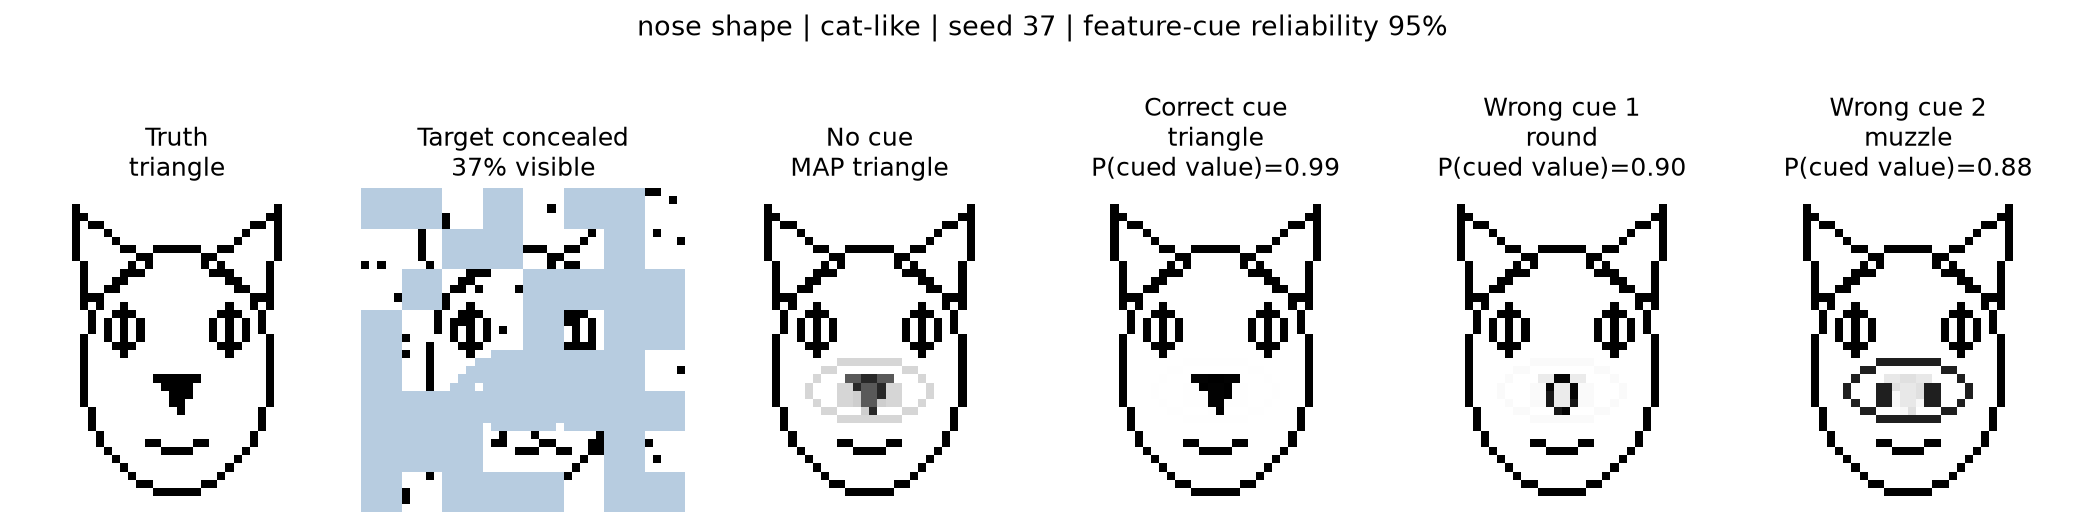
\includegraphics[width=\linewidth]{nose_concealed.png}\par\smallskip
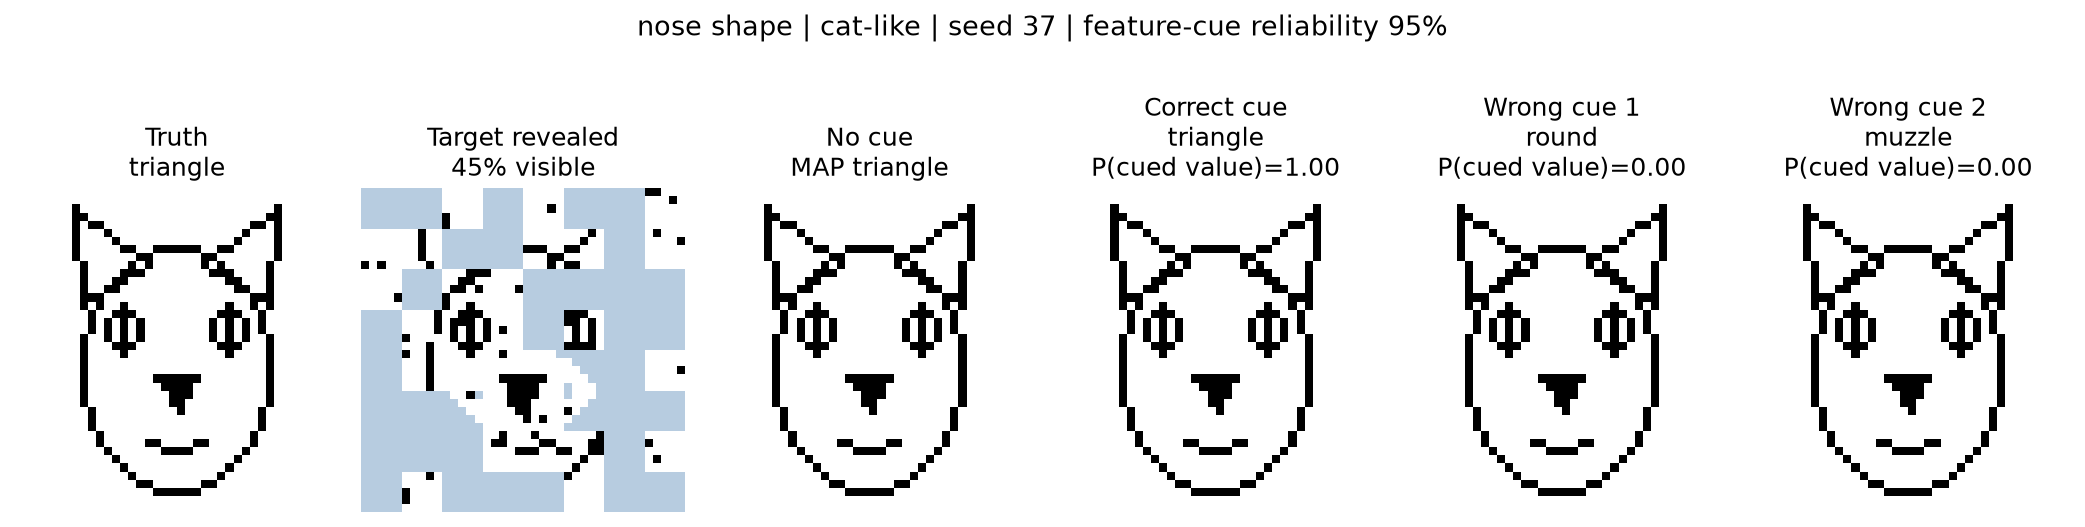
\includegraphics[width=\linewidth]{nose_revealed.png}
\caption{Direct nose cues on a cat-like drawing. The upper row conceals the pixels that distinguish nose alternatives. The lower row reveals those pixels. The four cue conditions show posterior-mean drawings. The probabilities refer to the indicated nose values.}
\label{fig:nose}
\end{figure}

\begin{figure}[htbp]
\centering
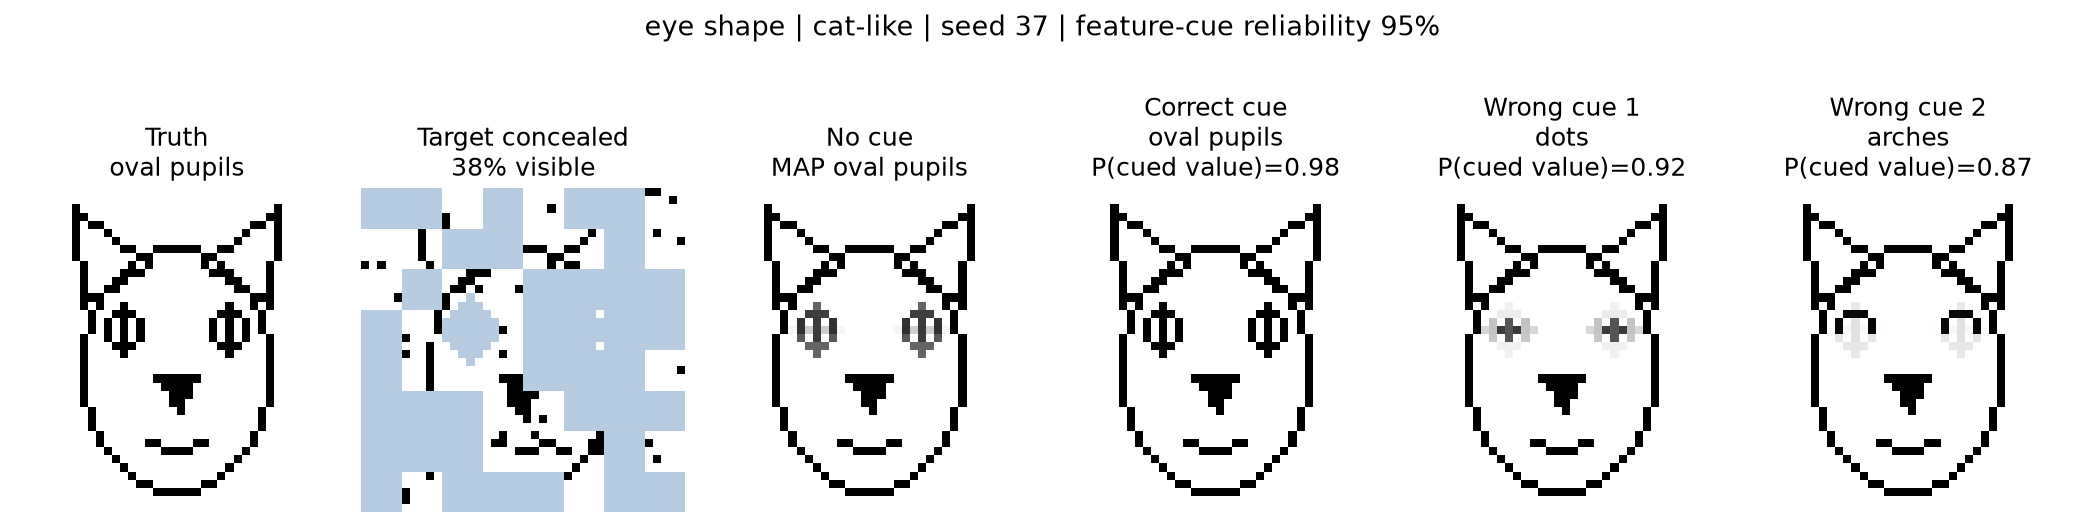
\includegraphics[width=\linewidth]{eye_shape_concealed.png}\par\smallskip
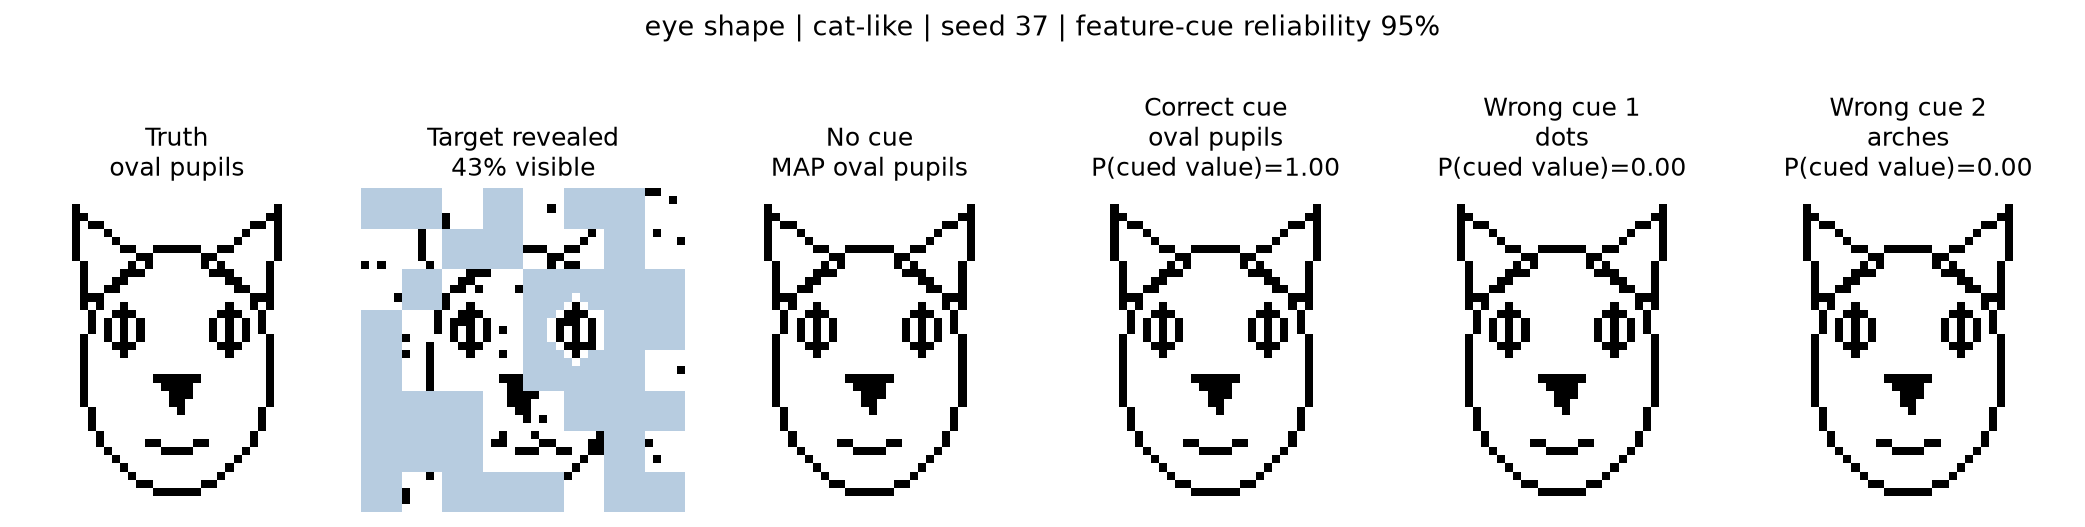
\includegraphics[width=\linewidth]{eye_shape_revealed.png}
\caption{Direct eye-shape cues on the same cat-like drawing. The upper row conceals the diagnostic pixels, and the lower row reveals them.}
\label{fig:eyes}
\end{figure}

\subsection{Matched comparison of learned priors}
Each method receives the same 840 masked test cases, with 12 held-out faces at each of ten visibility levels and seven correct-hint counts. The comparison uses the current renderer and a 5\% pixel-flip probability. Feature recovery counts how many of the six MAP feature values match the held-out recipe. Exact recovery requires all six to match.

\begin{table}[htbp]
\centering
\begin{tabular}{lrr}
\toprule
Prior & Mean features (of 6) & Exact recovery \\
\midrule
Labeled feature counts & 4.63 & 37.1\% \\
Supervised Hebbian & 4.63 & 37.1\% \\
Label-free competitive Hebbian & 4.58 & 37.1\% \\
Exemplar similarity & 4.89 & 40.8\% \\
Hopfield ($\tau=1$) & 5.45 & 66.5\% \\
Hopfield (exemplar-matched entropy) & 5.01 & 51.9\% \\
\bottomrule
\end{tabular}
\caption{Matched MAP recovery with $\alpha=12$. Competitive Hebbian scores average over three training initializations run on the same test cases.}
\label{tab:prior-comparison}
\end{table}

\begin{figure}[htbp]
\centering
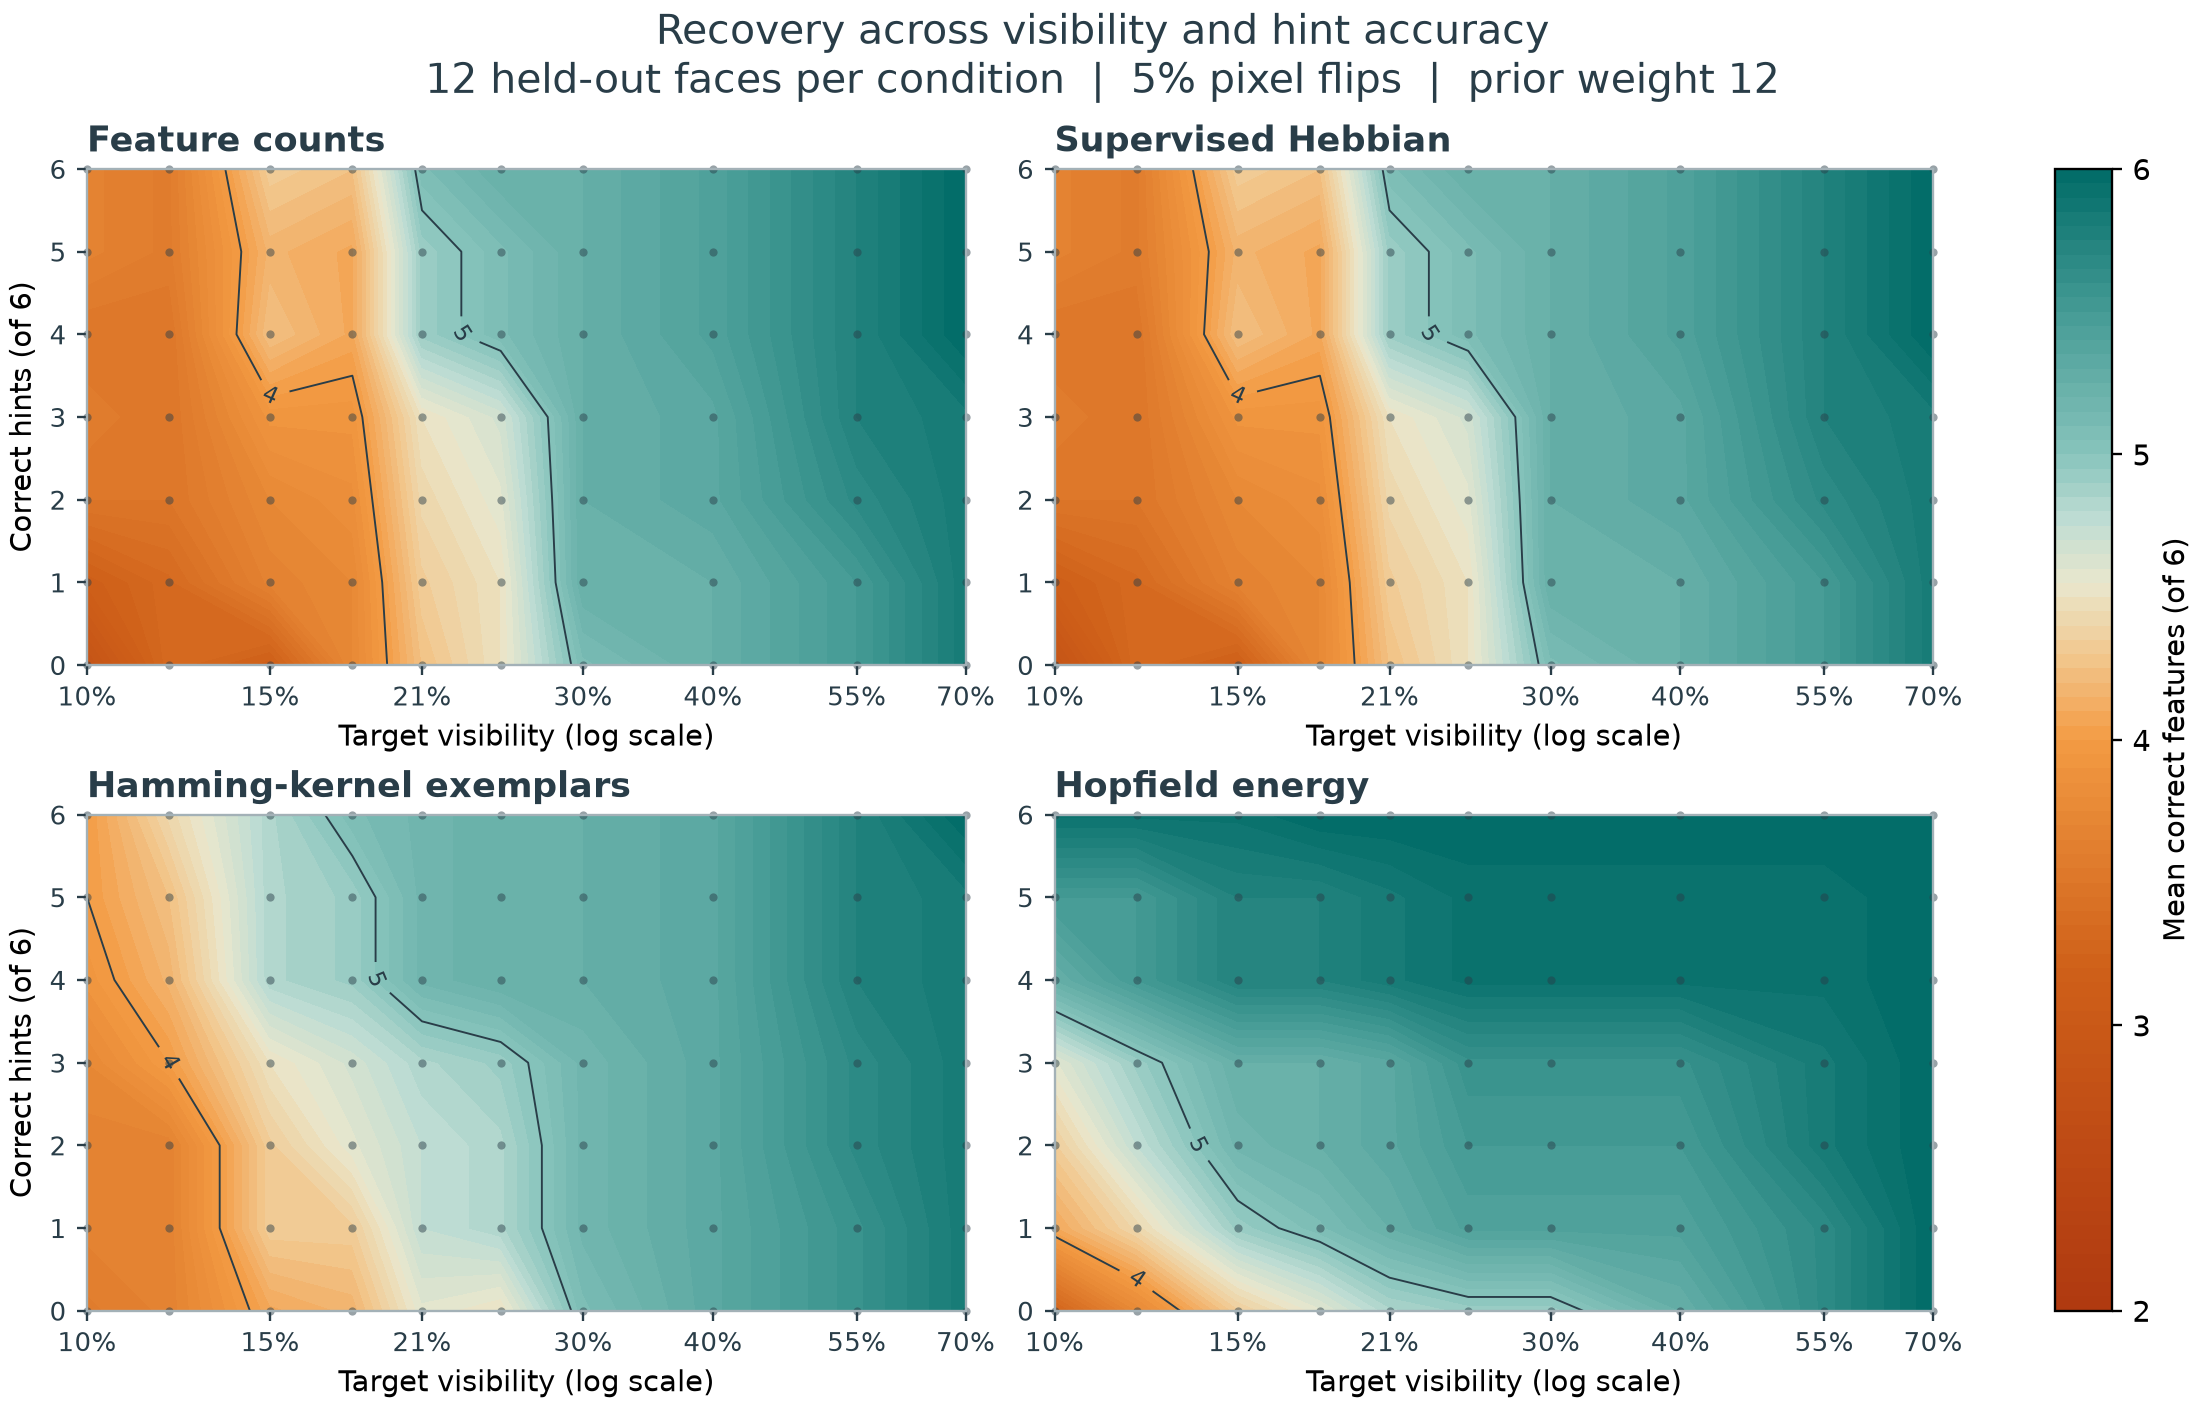
\includegraphics[width=\linewidth]{prior_contours.png}
\caption{Recovery across visibility and hint accuracy for the count, supervised Hebbian, exemplar, and Hopfield priors. All panels use the same trials.}
\label{fig:matched}
\end{figure}

The supervised update reproduces the counted prior, giving identical MAP choices. The label-free model averages 4.58 correct features, with individual seeds ranging from 4.55 to 4.65. The default Hopfield prior scores higher in this run. Its effective prior is also more diffuse than those of several comparators. Raising $\tau$ to approximately 3.626 matches the entropy of the weighted exemplar prior and reduces Hopfield recovery to 5.01/6. Using only image and hint scores ($\alpha=0$) gives an average of 5.50/6. These checks show how the apparent differences depend on prior strength.

\begin{figure}[htbp]
\centering
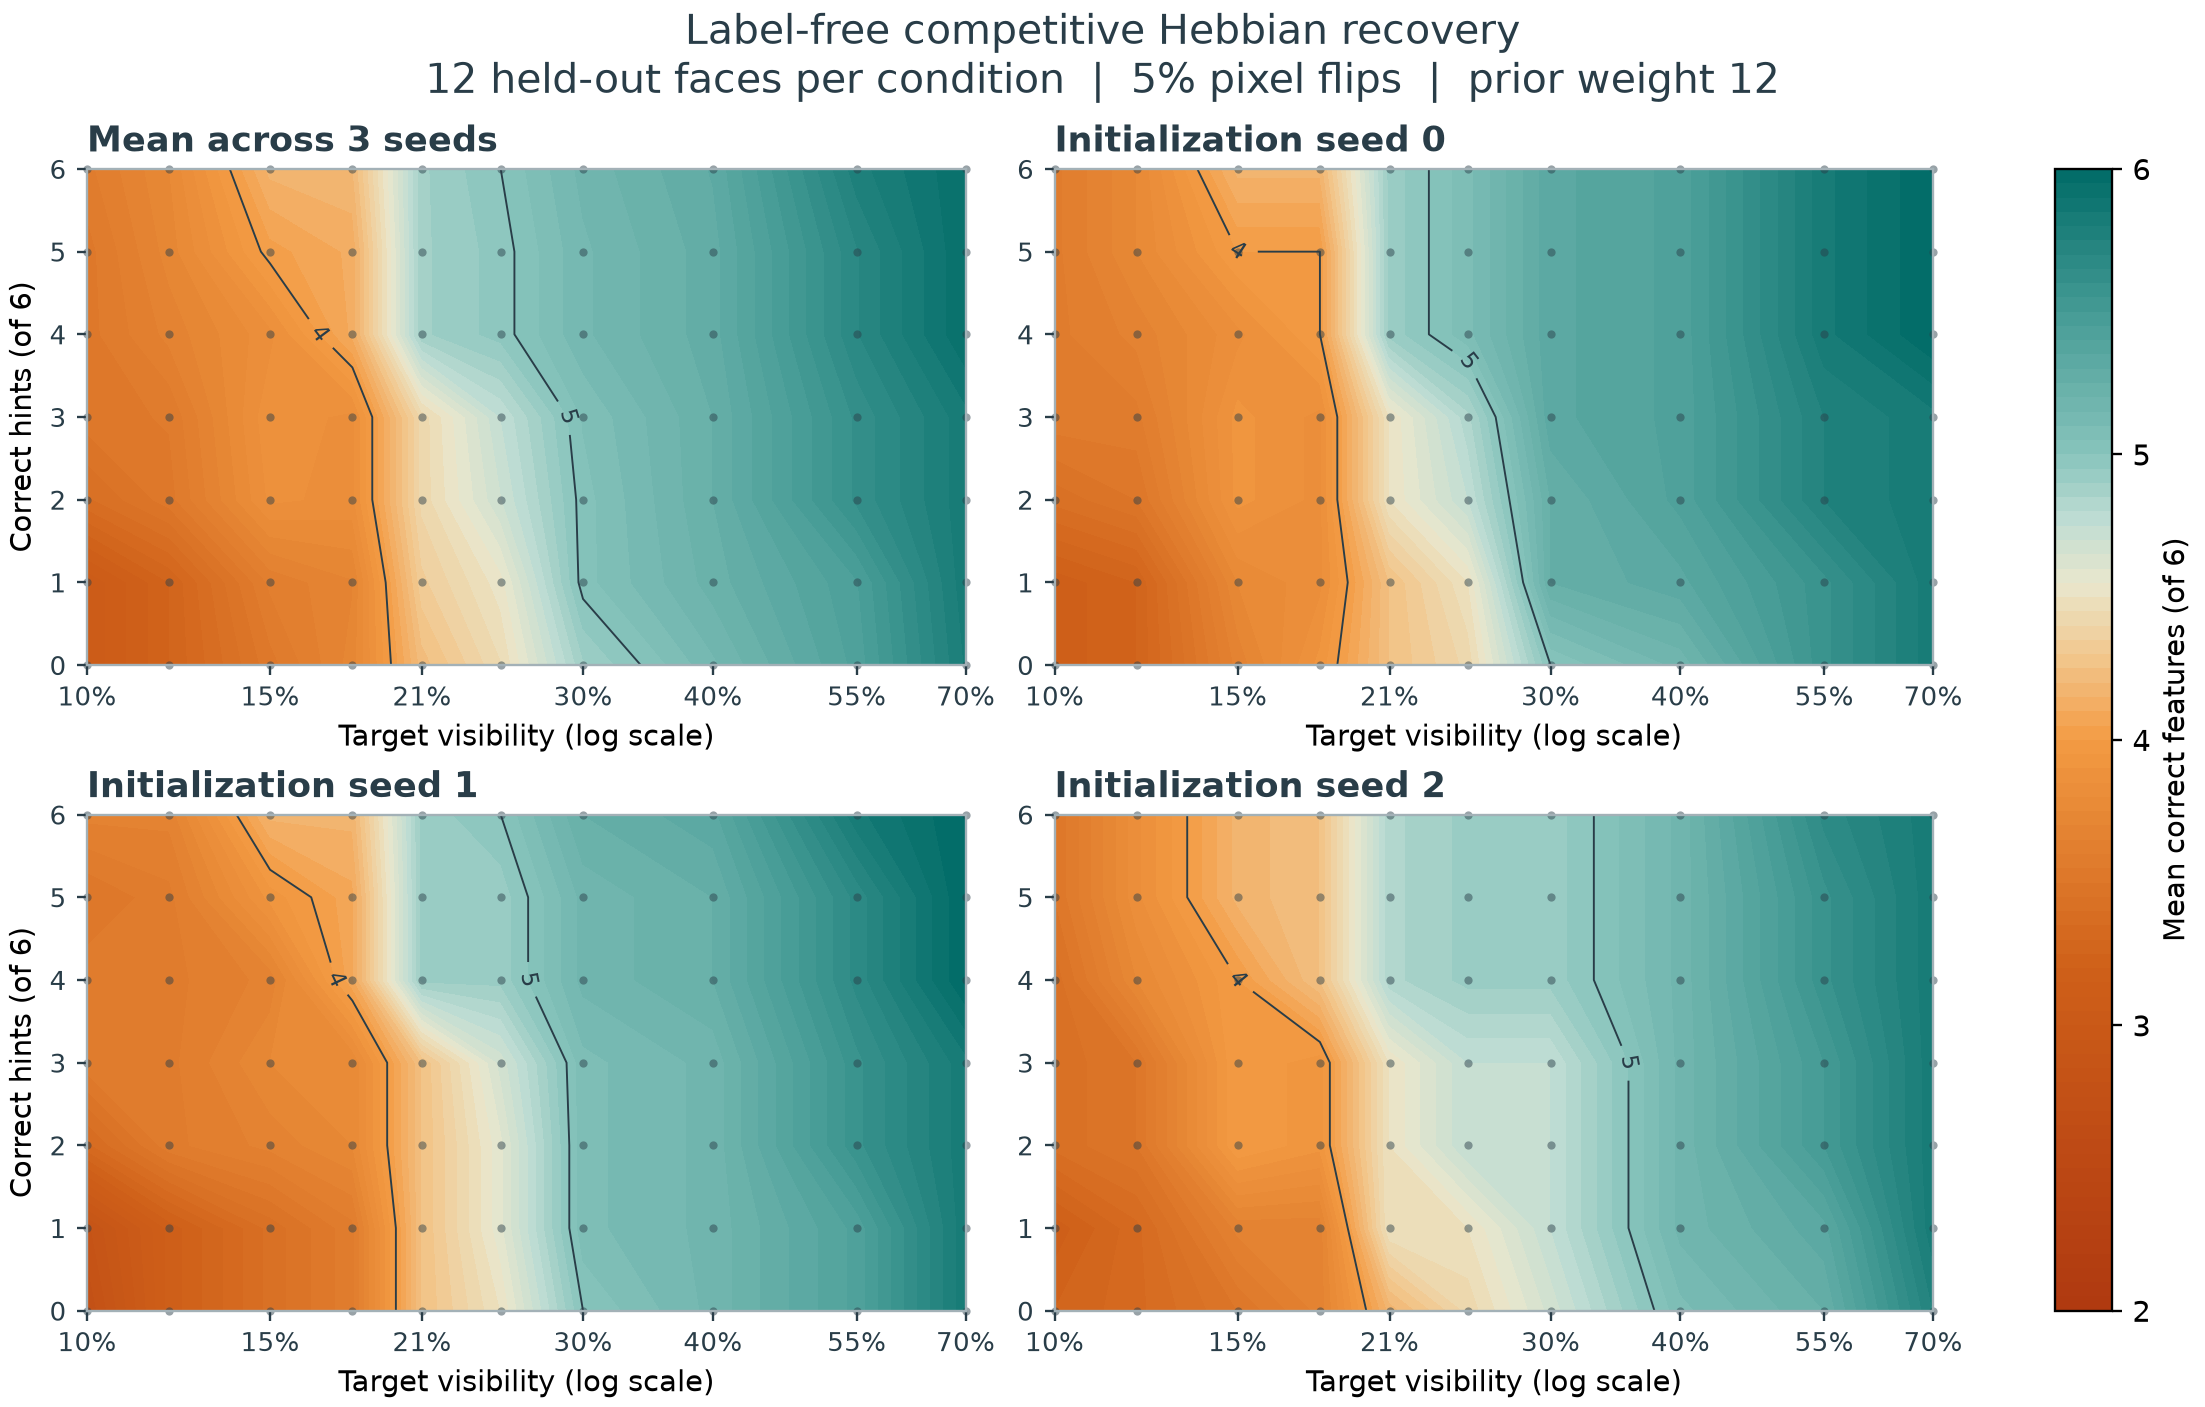
\includegraphics[width=\linewidth]{competitive_contours.png}
\caption{Label-free competitive Hebbian recovery on the matched trials, averaged over initializations and shown for each seed.}
\label{fig:competitive}
\end{figure}

\subsection{Label-free recovery across noise levels}
A second run varies target pixel flips across 2\%, 5\%, 10\%, 15\%, and 20\%, flipping a fixed number of randomly selected visible pixels in each trial. At each visibility, hint-count, and noise combination, 64 held-out faces are evaluated with the same three label-free fits. Across the 13 target visibilities, the average is 4.51 of 6 features. At the three visibility settings above 75\%, it is 5.56 of 6. At the 20\% flip setting, it is 3.72 of 6 across visibilities and hint counts.

\subsection{Reproducibility and interpretation}
The renderer and inference code are in \path{closure_model.py} and \path{vsa_inference.py}. The prior implementations are in \path{hebbian_prior.py} and \path{hopfield_prior.py}. The matched comparison uses \path{compare_experiment_priors.py}. The noise sweep and its high-visibility extension use \path{compare_capped_noise.py} and \path{extend_hebbian_visibility.py}. Their tables and settings are under \path{outputs/prior_comparison/}, \path{outputs/capped_noise_contours/}, and \path{outputs/capped_noise_high_visibility/}, respectively. The earlier seed sweep and targeted cues use the eye-shape vocabulary. Their saved metrics and case figures are in the original project's \path{outputs/seed_visibility_runs_2026-11-16/} and \path{outputs/targeted_feature_cues_2026-11-16/}.

These experiments reuse a small vocabulary, fixed centered images, and known masks. The targeted tests select masks to manipulate specific features' visual support. In the pilot with disclosed hint accuracy, people can use the count of correct hints to rule out recipes. The current computer comparison receives the hint values and uses an assumed per-hint reliability. The simulation also shares the same rendering rules between prior training and recovery. The results characterize how this particular model combines visible evidence and contextual input.

\section{Discussion on learning a cue-modulated encoder}
\subsection{The remaining question}
The present experiment shows how cues influence completion when recipes, feature meanings, and rendering rules are supplied. The broader question concerns the construction of those interpretations from ambiguous pixels. A cue such as ``cow face'' could help a system group disconnected regions into a head, assign a location to a muzzle, and identify which boundaries belong to the same part.

Cue specificity has multiple dimensions. ``Cow'' narrows an object category, while ``front-facing head'' constrains pose and part arrangement. A cue about a particular region can establish correspondence between an image patch and an object part. Testing these separately would clarify which information makes an initially ambiguous grouping usable. Studies of Mooney images already show effects of category-related and image-specific knowledge on recognition and contextual processing \cite{lazarova2025}.

\subsection{What pixel comparisons provide}
Ordinary pixel comparison evaluates agreement at corresponding image coordinates. The fixed VSA conversion packs those coordinate-specific values into a vector, allowing approximate comparison with cross-talk. Both methods obtain semantic feature interpretations through the supplied renderer and candidate recipes. Their grouping rules are implicit in the forward images we chose to generate.

A learned encoder could instead establish part membership, spatial correspondence, and feature evidence from the input. Grouping could make a nose representation depend on several separated patches and their relation to the surrounding head. It could also support movement, changes of pose, or variations in local appearance that fixed-coordinate matching handles only by adding more candidate renderings.

\subsection{A recurrent formulation}
One proposed extension maintains a spatial visual representation and a changing part-level belief state,
\begin{align}
v&=E_\theta(y,M),\\
h_{t+1}&=F_\theta(h_t,v,\operatorname{Cue}(c),e_t),\\
q_j^{(t)}&=\softmax(W_jh_t+b_j),\\
\widehat x_t&=D_\phi(q^{(t)},h_t),\qquad
e_t=M\odot(y-\widehat x_t).
\end{align}
Here, $E_\theta$ learns visual features, $F_\theta$ revises the interpretation using the cue and current prediction error, and $D_\phi$ predicts an image. Part-level spatial maps or attention weights would identify which pixels contribute to each inferred group. A nose prediction would then carry both a shape distribution and evidence about its location.

Training can use synthetic recipes and part masks to supervise the initial grouping problem, together with reconstruction of clean images. During testing, weights can stay fixed while the recurrent state changes. A differentiable renderer or learned decoder would permit reconstruction errors to train the inference process. Learned iterative inference and iterative object decomposition provide relevant computational precedents \cite{marino2018,greff2019}.

The cue effect should be evaluated within the encoder as well as at its output. For the same image, one could measure whether a cue changes the region assigned to the nose, the separation between competing shape representations, the number of refinement steps required, and the invention of unsupported boundaries. Training should include cue absence and controlled cue errors so that cue reliability is learned or specified.

\subsection{Where VSA and associative memory could contribute}
VSA could represent inferred part--property bindings and support queries for shape or position. A suitable encoder would need to produce representations with that factorization. Fixed random pixel codes alone establish coordinate identities, while the proposed learned grouping would establish correspondences between visual regions and part codes.

Sparse distributed memory could retrieve contextual associations or clean up a noisy part query if its address representation preserves relevant similarities. Recurrent unbinding and associative completion are also central to resonator approaches to VSA factorization \cite{frady2020}. These components could be tested after a cue-sensitive grouping model is established. Their contribution would be evaluated against the same encoder with an ordinary vector representation.

The practical next test is whether a learned recurrent encoder can improve part grouping as cue information becomes more specific while retaining appropriate uncertainty and responding to contradictory pixels. This addresses the original question about when a patch becomes interpretable as a possible muzzle.

\begin{thebibliography}{9}
\bibitem{schwiedrzik2018}
C. M. Schwiedrzik, L. Melloni, and A. Schurger.
Mooney face stimuli for visual perception research.
\emph{PLOS ONE}, 13(7), e0200106, 2018.
\href{https://doi.org/10.1371/journal.pone.0200106}{doi:10.1371/journal.pone.0200106}.

\bibitem{lazarova2025}
Y. Y. Lazarova, Y. Huang, L. F. Muckli, and L. S. Petro.
Perceptual priors update contextual feedback processing in V1.
\emph{Topics in Cognitive Science}, published online 2025.
\href{https://doi.org/10.1111/tops.70018}{doi:10.1111/tops.70018}.

\bibitem{marino2018}
J. Marino, Y. Yue, and S. Mandt.
Iterative amortized inference.
\emph{Proceedings of ICML}, PMLR 80, pp. 3403--3412, 2018.
\url{https://proceedings.mlr.press/v80/marino18a.html}.

\bibitem{greff2019}
K. Greff et al.
Multi-object representation learning with iterative variational inference.
\emph{Proceedings of ICML}, PMLR 97, pp. 2424--2433, 2019.
\url{https://proceedings.mlr.press/v97/greff19a.html}.

\bibitem{frady2020}
E. P. Frady, S. Kent, B. A. Olshausen, and F. T. Sommer.
Resonator networks for factoring distributed representations of data structures.
arXiv:2007.03748, 2020.
\url{https://arxiv.org/abs/2007.03748}.
\bibitem{li2006}
P. Li, T. J. Hastie, and K. W. Church. Very sparse random projections. KDD, 2006.
\url{https://web.stanford.edu/~hastie/Papers/Ping/KDD06_rp.pdf}.

\bibitem{compressive2012}
Target detection performance bounds in compressive imaging. EURASIP Journal on Advances in Signal Processing, 2012, article 205.
\url{https://doi.org/10.1186/1687-6180-2012-205}.

\bibitem{frady2018}
E. P. Frady, D. Kleyko, and F. T. Sommer. A theory of sequence indexing and working memory in recurrent neural networks. Neural Computation, 2018.
\url{https://arxiv.org/abs/1803.00412}.
\end{thebibliography}
\end{document}
